\chapter{提案するシステム}
\label{chap:method}
本章では,提案するシステムについて述べる.
提案するシステムでは,人間が作成した「次の角まで直進.左折.」などのシナリオから
指示された道順に従い,カメラ画像に基づいて目的地まで自律移動する.
〜で提案するシステムの概要と一連の内容を述べた後,システムを構成する
モジュールについて詳細に述べる.
%
%\input{introduction/preface}
%
\section{提案システムの概要}
〜に提案するシステムの概要とシステムにより,ロボットが目的地まで
自律移動する一連の流れを示す.
提案するシステムは〜で述べるシナリオモジュールと
〜で述べる経路追従モジュール
〜で述べる通路分類モジュールの
3つのモジュールで構成されている.
これらのモジュールはROS
機械学習のフレームワークとしてpytorch
CUDAを使用している
ロボットはaからdの一連の流れにより指示された道順に従って目的地まで自律移動する.



\section{経路追従モジュール}
経路追従モジュールについて述べる.
このモジュールは,事前に 模倣学習させた環境で,
カメラ画像に基づいて経路を 追従するモジュールであり,
分岐路では入力された目 標方向によって経路を選択して走行する.
〜に経路追従モジュールのシステムを示す.
データセットに動的に変化させるやつ
積極的な蛇行オーバーサンプリングの話

\section{通路分類モジュール}
通路分類モジュールについて述べる.
このモジュールは,シナリオの「条件」が満たされたかの判定に必要な
通路の特徴を,カメラ画像を入力として分類する.
使用するカメラについては,経路追従モジュールと同様に,データセットの収集時は3つ
学習後は1つである.
通路の特徴の分類は,島田らの手法に倣い,\ref{fig:class}に示す8つとしている.
% この中で,突き当たりは
% 行き止まり,角(右),角(左),三叉路(中央)
% 右手に通路が〜角(右)十字路 三叉路(右)三叉路(中央)
% 左手に通路が〜角(左)十字路 三叉路(中央)三叉路(左)
\begin{figure}[htbp]
    \centering
     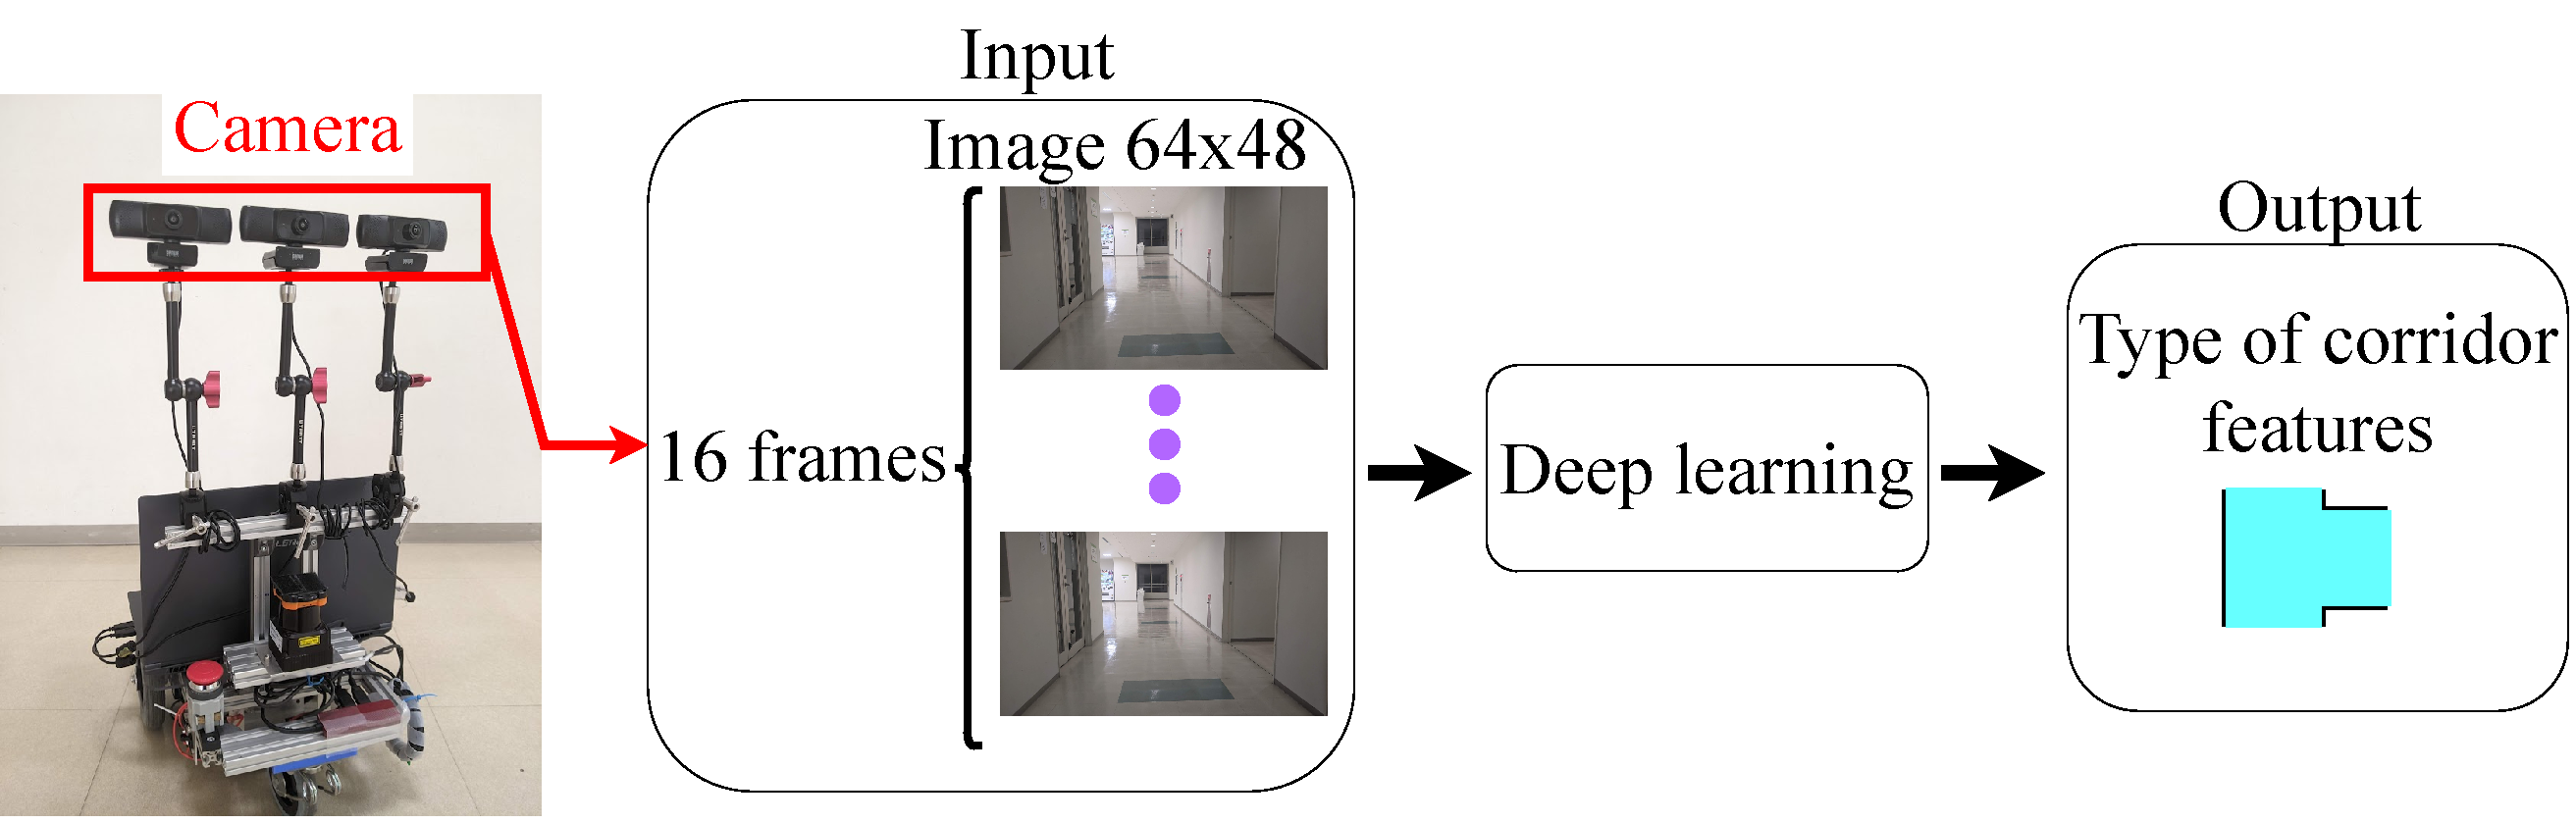
\includegraphics[width=100mm]{images/pdf/intersection_abs.pdf}
     \caption{Path-following module system Quoted from \cite{haruyama2023}}
     \label{fig:intersection_abs}
\end{figure}
\begin{figure}[htbp]
    \centering
     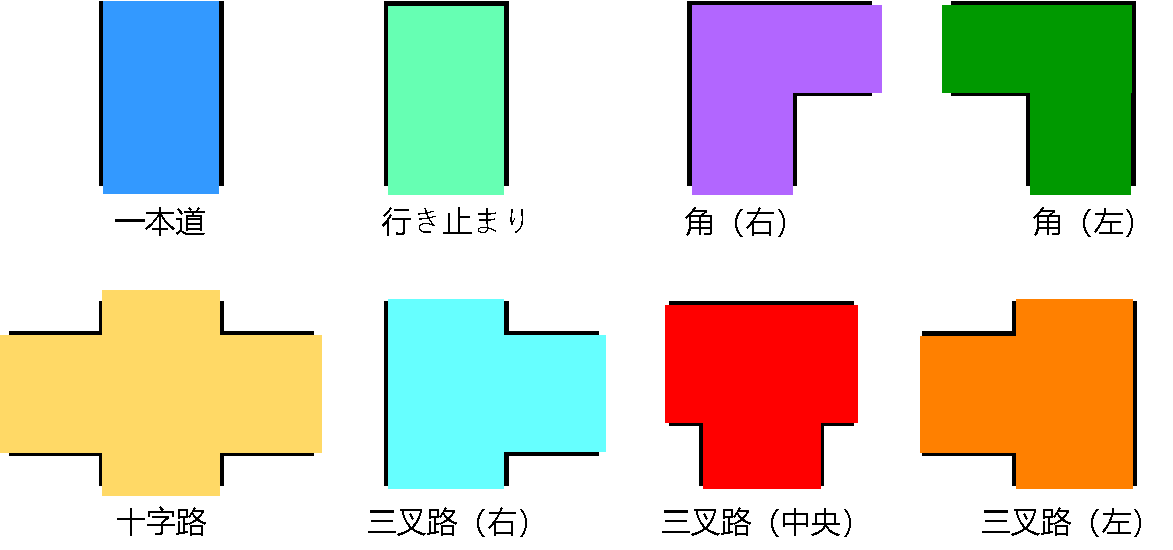
\includegraphics[width=100mm]{images/pdf/class.pdf}
     \caption{Path-following module system Quoted from \cite{haruyama2023}}
     \label{fig:class}
\end{figure}
\newpage

ネットワークの構成を\ref{fig:int_net}に示す.
このネットワークアーキテクチャはDhaivat らが提案するCNNとLSTMを組み合わせた
IntersectNet[7] に倣って構築した.
なおCNNアーキテクチャは実時間性の観点からAlexNetからMovileNetV3-Largeへ変更している.

ネットワークはフレーム数 16,画像サイズ64×48の連続したRGB画像データを入力とする.
画像データは各フレームごとにCNNで処理され,この特徴ベクトルはLSTMへ入力される.
各LSTMの出力は分類層(全結合層)へ渡される.
最後に,全ての分類層の出力を融合層へ渡し,融合層は入力の平均を取ることで,
最終的な分類結果を出力する.
損失関数としてCrossEntropyLoss,活性化関数にはAdamを使用する.
\begin{figure}[htbp]
    \centering
     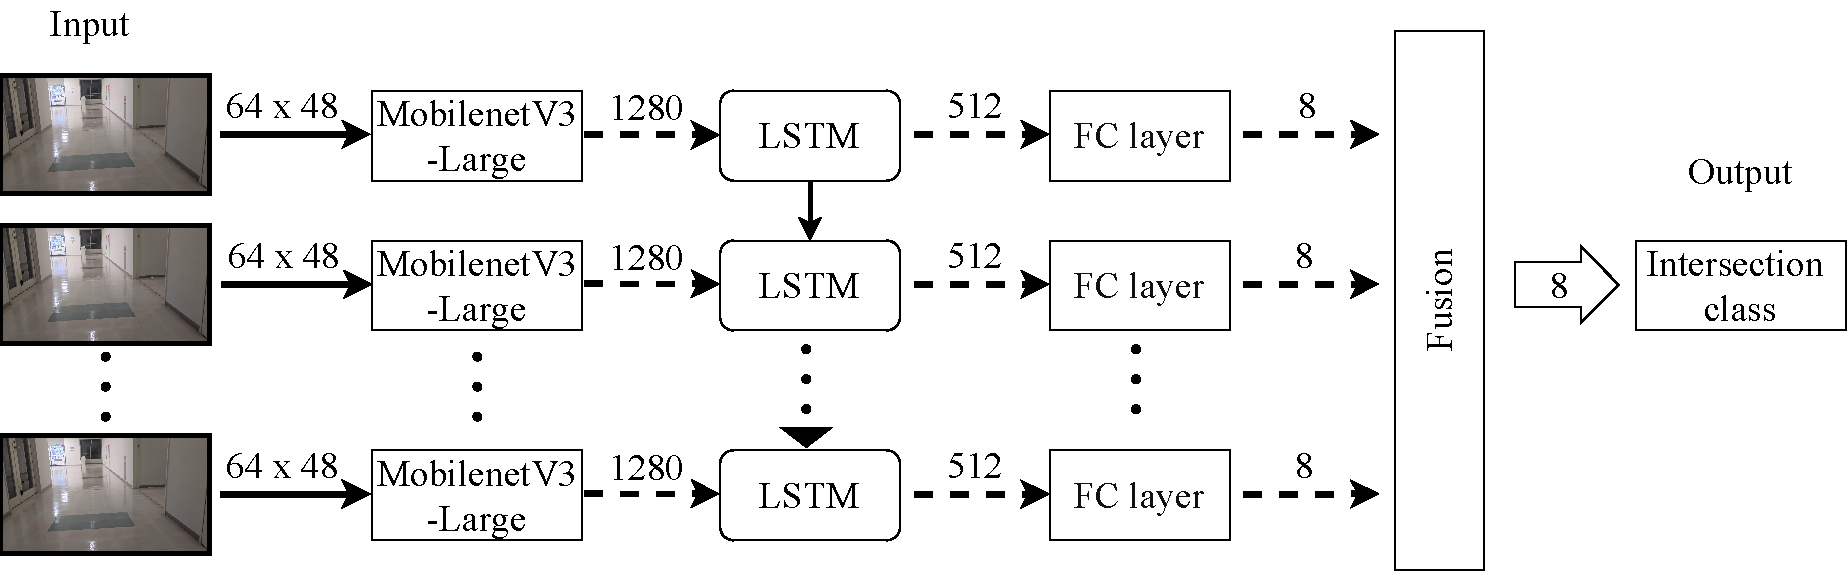
\includegraphics[width=120mm]{images/pdf/network-intersect.pdf}
     \caption{Path-following module system}
     \label{fig:int_net}
\end{figure}

次に通路分類モジュールのデータセットの作成について述べる.
データの作成では,経路追従モジュールの学習と同様に,
メトリックマップに基づいたルールベース制御器によって経路を走行する.
その際,フレーム数 16 の連続したカメラ画像と通路の分類ラベルを1組とし,
0.125秒周期でデータセットへ加える.分類ラベルのアノテーションは,
\ref{fig:int_net}に示すように,通路の特徴を予めメトリックマップに登録しておくことで,自動的に行う.
\begin{figure}[htbp]
    \centering
     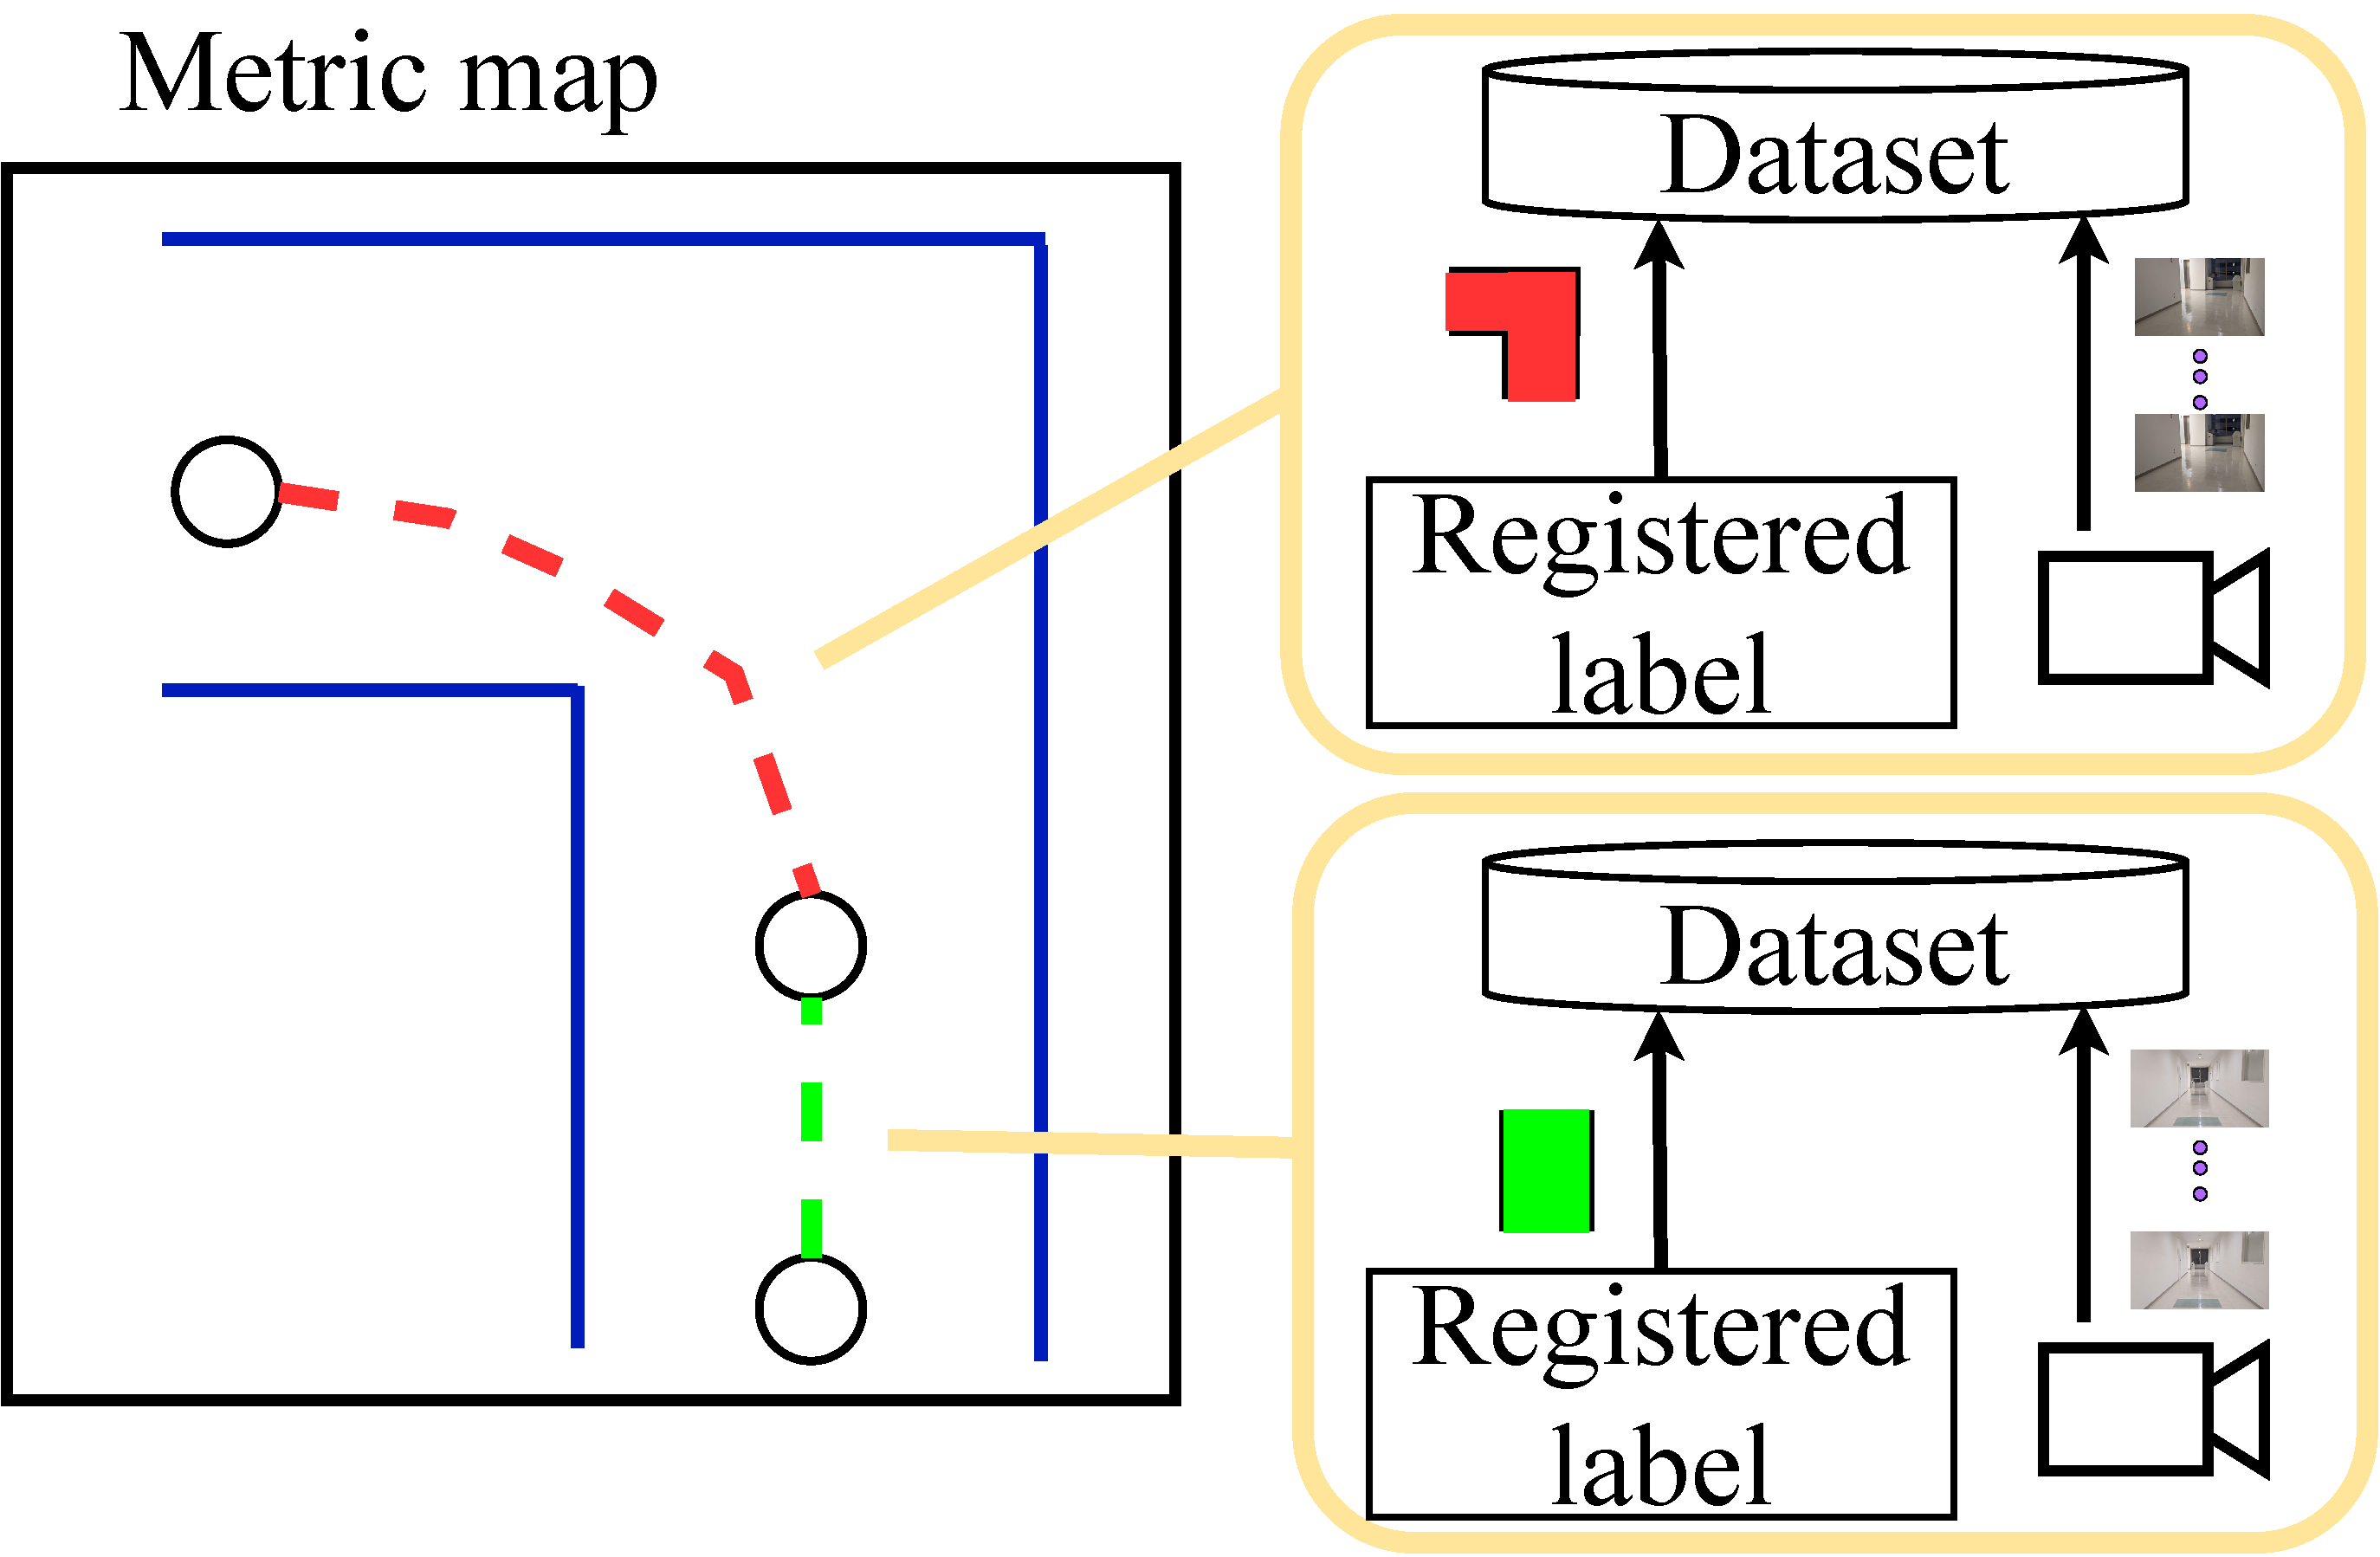
\includegraphics[width=100mm]{images/pdf/map_label.pdf}
     \caption{Path-following module system}
     \label{fig:int_net}
\end{figure}
\newpage
学習するデータセット内で,各クラスのデータ数か
大きく異なる不均衡データは,分類結果に大きな影響を与える
とされている. 経路追従モジュールではオーバーサンプリングを行ったが,
そのため,本稿では学習する際に,
データセット内のクラス間のデータ数によって重
み付けを行うコストアプローチを導入している.
具体的には,損失関数である損失関数(CrossEntropyLoss)で用いる
クラスごとの重みをメジャーデータを基に決定する.
\section{シナリオモジュール}
シナリオモジュールについて述べる.
シナリオモジュールはトポロジカルマップから作成されたシナリ
オから「突き当りまで」という「条件」や「左折」なとの「行動」を解釈し,
単語で構成された経路を分岐路 での目標方向へ変換して出力する.

\ref{fig:topo2sce}にトポロジカルマップとそれをもとに作成されるシナリオを示す.
図の例では出発地点をエッジ2,目的地をノード2として,その間のエッジとノードを移動する.
エッジ2からノード1は「三叉路まで」という条件と「直進」という行動,
ノード1からエッジ1は「右折」という行動,
エッジ1からノード2は「突き当り(三叉路)まで」という条件と「直進」の行動で表現される.
これらを統合すると,
最終的に「三叉路まで直進.右折.突き当たりまで直進.停止.」
のシナリオが作成される.

次に作成したシナリオを目標方向に変換する処理を述べる.
シナリオを句点ごとに分解し,部分シナリオというものを作成する.
この部分シナリオには次の部分シナリオに遷移するための「条件」とロボットが行う必要がある「行動」
が含まれている.
この部分シナリオを形態素分析(MeCab\cite{2004ConditionalRF})を用いて単語へ分割する.
次に分割した単語を,予め作成した「条件」と「行動」にまつわる,
以下の項目の辞書と照らし合わせ,一致したものを抽出する.
\begin{figure}[htbp]
    \centering
     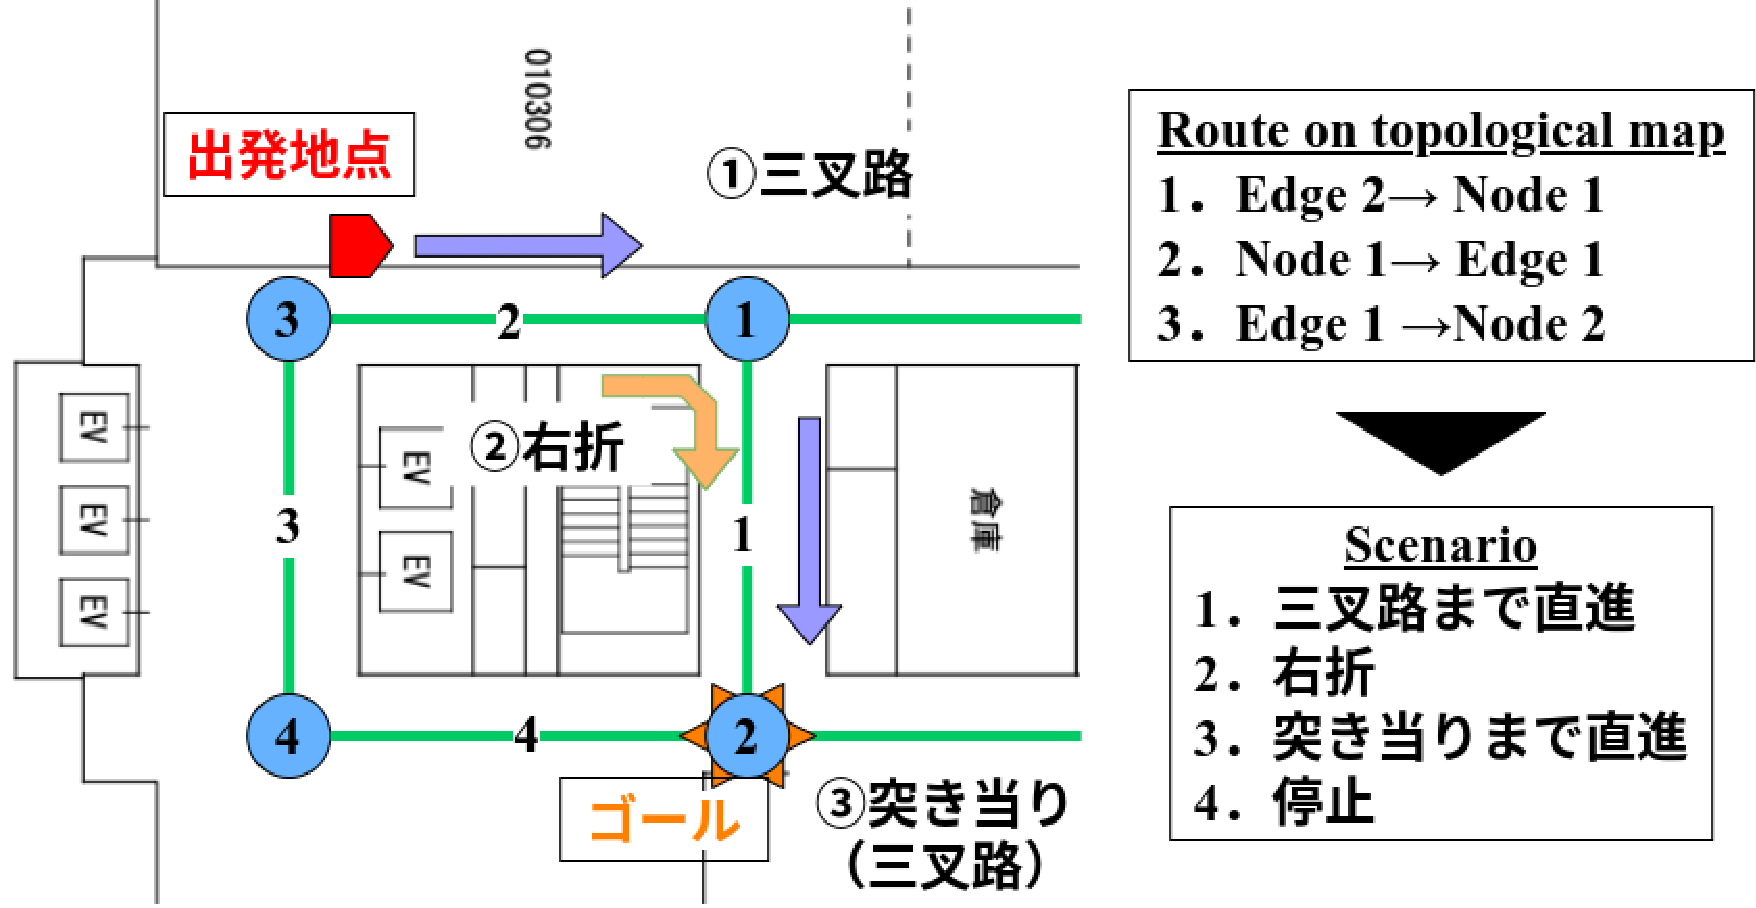
\includegraphics[width=90mm]{images/pdf/topo2sce.pdf}
     \caption{Path-following module system Quoted from \cite{haruyama2023}}
     \label{fig:topo2sce}
\end{figure}

\begin{enumerate}
    \item [1)] 通路の特徴 例えば,「三叉路」「角」など
    \item [2)] 順番 例えば,「3 つ目の」「2 番目の」など 
    \item [3)] 方向 例えば,「左手に」「右手に」など
    \item [4)] 行動 例えば,「右折」「停止」など
\end{enumerate}
% 1)通路の特徴 例えば,「三叉路」
% 「角」など 2)順番 例えば,「3 つ目の」「2 番目の」など 
% 3)方向 例えば,「左手に」「右手に」など 4)行動 例えば,「右折」「停止」など
先に示した例は句点ごとに,
三叉路まで直進/ 
右折/   
突き当たりまで直進/  
停止/ 
と分解される.

1つ目の条件と行動は 
1)通路の特徴 三叉路,4)行動 直進,

2つ目の行動は 4)行動 右折となる.

3つ目の条件と行動は
1)通路の特徴 突き当たり 4)行動 直進

4つ目の行動は
4)停止となる.

これらの4)行動を〜で示したベクトルで表現し,分岐路での目標方向として,経路追従モジュールへ与える.
ここで,「三叉路まで」といった条件を達成したかの判定は,
〜の通路分類モジュールの分類結果を用いて行う.

%
